\documentclass[asi]{picINSA}
\usepackage{cite}

\begin{document}

    \titreGeneral{Bibliographie}
	\sousTitreGeneral{\newline Sujet RPG 1}
	\titreAcronyme{\LARGE IHME}
	\version{1.00}
	\referenceVersion{bibliographie}
	
	\couverture{}

\tableofcontents{}

\chapter*{Introduction}

Un des challenges principaux de développeur de jeux vidéos est la crédibilité de leurs personnages non joueurs et 
de leurs réactions. Pour que les réactions des personnages soient réalistes, il s'agit de bien les modéliser pour 
qu'il puissent donner l'illusion d'être vivant ~\cite{Bates94therole}. De plus, dans les jeux vidéos le joueurs,
n'est pas simplement spectateur mais bien acteur dans le scénario. Si les réactions du joueur sont imprévisibles,
cela signifie qu'il faut générer un nouveau scénario en cas d'action imprévue du joueur, ou d'un personnage non joueur.

Nous aborderons d'abord le problème de la création d'un personnage réaliste puis les difficulté de la création de scénario.
Enfin nous aborderons les applications possibles sur notre projet et nous conclurons.

\chapter{Création des personnages}
~\\
Il y a plusieurs approches possibles pour rendre les personnages intéressant dans la narration interactive. Nous allons d'abord voir comment sont représentées les actions des personnages non joueurs (PNJ), et comment un joueur peut agir dessus. Nous verrons ensuite comment modéliser la personnalité des personnages, pour agir automatiquement sur le choix des actions d'un PNJ.\\


\section{Interactions humain-personnage}

Dans ~\cite{IRIS:conf/aamas/CavazzaCM2002}, le principe repose sur une histoire qui se déroule sous les yeux d'un joueur humain. Celui-ci peut à tout moment décider d'intervenir, en agissant dans la scène (ex : déplacement d'un objet), ou bien en donnant des conseils ou des indications à un PNJ. Leur système utilise une reconnaissance vocale pour interprêter ce que le joueur veut dire au PNJ. Ce message est ensuite transformé pour être compris par le PNJ, qui va changer son comportement en fonction. Par exemple, si le PNJ cherche un objet mais ne le trouve pas dans la pièce où il se trouve, le joueur peut lui donner une indication, il va donc aller au bon endroit.\\

Les actions du personnages sont représentées par un HTN : Hierarchical Task Networks. (voir figure \ref{fig:htn})\\
\begin{figure}[h!]
  \centering
  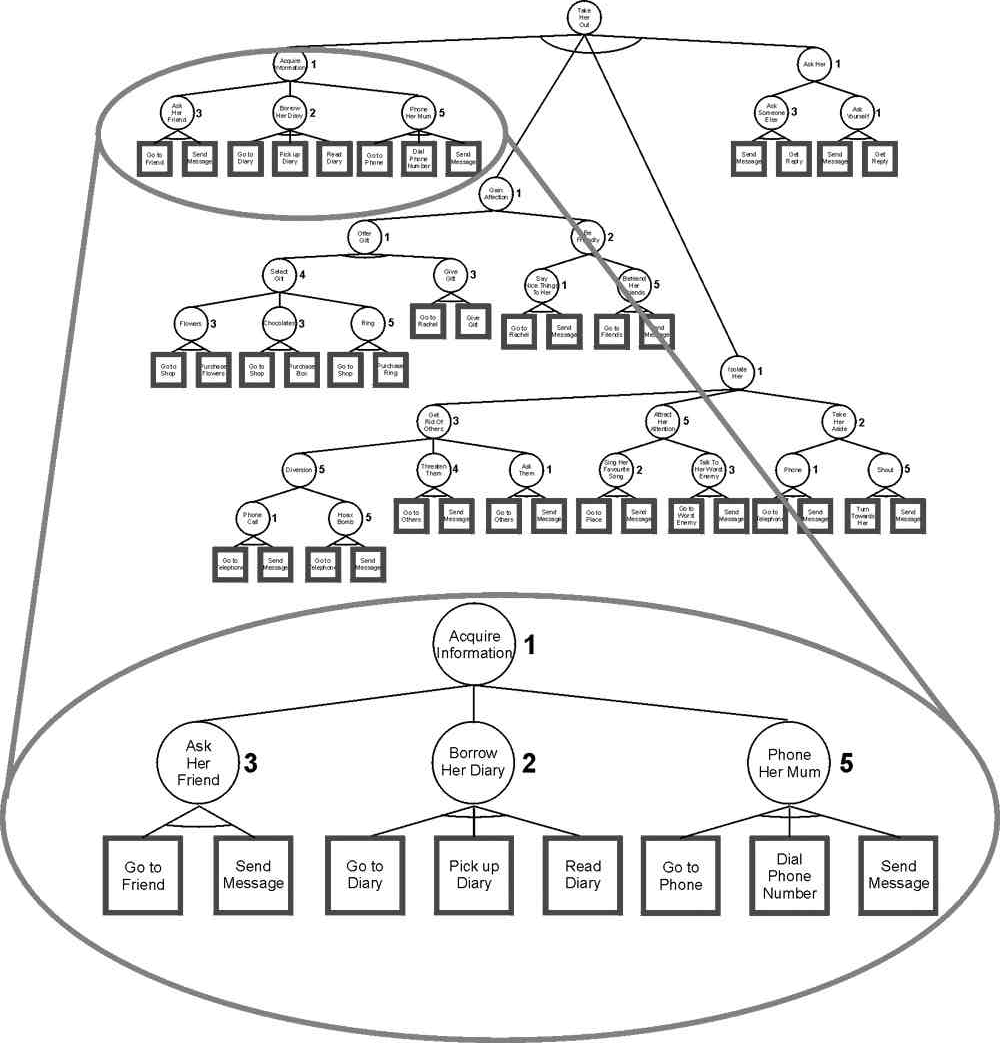
\includegraphics[scale=0.4]{images/htn.png}
  \caption{Hierarchical Task Networks}
  \label{fig:htn}
\end{figure}

La racine de cet arbre contient l'objectif principal du PNJ. Les noeuds en dessous sont les différents sous-objectifs nécessaires à court terme pour réaliser l'objectif principal. Pour chaque sous-objectif, une liste d'actions possible à effectuer pour le réaliser donne au PNJ différents moyens d'arriver à ses fins. Le choix dans ces actions s'effectue pour chaque sous-objectif en prenant les actions de gauche à droite, et si la première action est impossible, on prend la suivante, etc. Un poids peut être associé à chacune de ces actions pour éviter un choix qui pourrait être mal perçu par les autres personnages par exemple.\\


\section{Modélisation de la personnalité}

Dans un jeu vidéo, beaucoup d'éléments peuvent être scriptés pour faire réagir les PNJs d'une certaine façon. En revanche, en laissant le joueur assez libre dans ses actions, il faut trouver un autre moyen pour que les PNJs réagissent automatiquement, que ce soit par leurs actions directes, ou les émotions qu'ils laissent paraîtres.\\

\subsection{Relations sociales}

Comme présenté dans ~\cite{IRIS:conf/aiide/OchsSC2008}, la plupart des jeux de rôles ou des jeux d'aventures plongent le joueurs dans un rôle précis, avec un contexte déjà établi. L'impact des actions du joueurs sont alors généralement simplifiés a :

\begin{itemize}
\item un alignement : bien ou mal, loyal ou chaotic, pouvant limiter
  les actions possibles du joueur ou générer différentes réactions de
  la part des PNJs

\item une réputation, connu de tous les PNJs, qui peut modifier
  l'attitude de ceux-ci envers le joueur (par exemple, un joueur avec
  une mauvaise réputation pourra se faire attaquer dès qu'il croisera
  un garde).
\end{itemize}

~\\
Des résultats tirés d'études psychologique peuvent être utilisés afin de représenter plus précisément les relations sociales. Dans la plupart des travaux précédents, les chercheurs se sont basés sur un modèle statique : la relation entre une émotion ressentie et la réaction d'un personnage était fixé. Nous allons voir ici un modèle de relations sociales dynamique, connecté à un modèle lié aux émotions : les émotions générées pendant une interaction peuvent produire différentes réactions, selon l'état du personnage et les émotions qu'il ressent.\\

Il n'existe pas de règles sur le nombre de variables nécessaires pour caractériser les relations sociales, mais on peut en ressortir 4 principales : 
\begin{itemize}
\item l'appréciation entre 2 personnages,
\item la dominance : la force qu'un personnage peut exercer sur un autre,
\item la solidarité : les ressemblances entre 2 personnages,
\item la familiarité, utile pour faire varier le type et la quantité d'information partagé.
\end{itemize}
Il faut savoir que les relations sociales sont orientées et pas nécessairement symétriques.\\

Pendant une interaction, les émotions ressenties par les 2 interlocuteurs peuvent changer leurs relations. En utilisant un modèle émotionnel, on représente l'état émotionnel par 4 vecteurs (sur [-1;1]) :
\begin{itemize}
\item joie / angoisse,
\item espoir / peur,
\item admiration / reproche,
\item fierté / honte.
\end{itemize}
Chacun des ces vecteurs vont agir positivement ou négativement sur les relations entre les personnages.

\subsection{Émotions}

Comme nous pouvons le voir dans ~\cite{IRIS:conf/aiide/Eladhari2010}, des recherches ont été faites afin de créer un prototype de monde de jeu multijoueur. Dans celui-ci, la personalité des personnages est la base de tout le fonctionnement. Chaque personnage possède des attributs de personnalité, et les joueurs voulant rejoindre ce jeu doivent passer un test afin de déterminer leurs caractéristiques propres.\\

Pour faire ceci, ils utilisent un \rq{}Mind Module\lq{} (\textit{module d'esprit}), un agent semi-autonome représentant l'architecture de l'esprit des personnages. Il se base sur 4 types d'éléments : les traits, les émotions, les sentiments et l'humeur.\\
\begin{itemize}
\item Les traits représentent la personnalité de base d'un personnage, et avec une certaine relation avec les émotions, cela peut affecter la force avec laquelle un personnage va ressentir les événements.
\item Les émotions représentent l'état d'esprit du personnage.
\item Les sentiments permettent de créer des liens entre les entités du monde. Cela peut agir sur les résultats d'un événement par exemple.
\item L'humeur est séparée en 2 partie : l'humeur intérieure, c'est-à-dire la façon dont un personnage se sent, et extérieure, ce qu'il va montrer aux autres.
\end{itemize}
~\\
Ces éléments ne sont pas tous modifiés de la même façon. En effet, les traits sont fixés lors de la création du personnage et ne changeront pas. Les émotions ressenties vont diminuer rapidement quelques minutes après l'événement déclencheur. À l'inverse, l'humeur peut rester pendant plusieurs heures.

\chapter{Génération de l'intrigue}

\section{Narration automatisée}

Au temps où les jeux vidéos n'existaient pas, les recherches se concentrait sur la grammaire et sur la création d'intrigue, c'est à dire sur la génération de texte. Cet aspect n'est pas inintéressant dans l'optique d'un jeux vidéo, car il peut être nécessaire de faire dialoguer les PNJ, voir leur faire raconter une histoire à partir d'un événement généré.


\subsection{Principe de la narration automatisée}

La génération de scénario est basé sur l'ordonnancement temporel des différentes scènes à partir d'une structure sémantique de base ~\cite{cavazza2002character}. Elle est décomposée en deux éléments par l'école formaliste Russe ~\cite{Callaway2002213} : la fabula et le suzjet. 

\subsubsection{Fabula}

La fabula est la connaissance du monde dans lequelle se déroule la narration. Cette structure sémantique de base, une ontologie, est ce qui permet de savoir comment interagissent chaque objets et personne du monde. La fabula est la somme de tout les objets du monde permet de générer le flux narratif. \\

La fabula est le suzjet peuvent être distingué car pour une même ontologie on peut obtenir une infinité d'histoire différentes en faisant varier l'ordre de présentation et de même des modifications dans l'ontologie permettent de changer le résultat.

\subsubsection{Suzjet}

Le suzjet est en quelque sorte le style du narrateur. Le choix de l'ordre de présentation, de la syntaxe utilisée, et de la décision de cacher ou non une information, par exemple dans le cas d'un mystère sont extrémement important. Avoir une bonne ontologie ne suffit pas si le narrateur se contente d'énumérer les faits présent à l'intérieur. \\
Par exemple, dans le cas d'un roman policier si le meurtrier était dévoilé dès le début, la narration serait de mauvaise qualité. Il est donc nécessaire d'évaluer la qualité d'une narration.

\subsection{Evaluation de la qualité d'une narration}

Le meilleur juge de la qualité d'un texte est un être humain, la plupart des évaluations sont donc réalisées par des êtres humains ~\cite{Callaway2002213}. Nous allons donc aborder quels sont les différents critères permettant d'évaluer la qualité d'une narration.

\subsubsection{Cohérence de l'intrigue}

La cohérence de l'intrigue est la pertinence de l'intrigue générée par le narrateur tout au long de l'histoire. Le narrateur doit donc se baser sur une fabula cohérente mais égélement sur un suzjet cohérent. Il est donc nécessaire que le narrateur choisisse un genre ~\cite{Ciarlini:2010:ERP:1658866.1658874} pour que son style soit reconnaissable.

\subsubsection{Réalisme des personnages}

Les personnages sont réaliste si le spectateur ou le lecteur peut penser que les actions réalisées par un personnage sont influencées par sa personalité et par ses émotions. Par exemple, il paraîtrait illogique qu'une informaticienne introvertie ait envie de faire la tournée des bars pour draguer plutôt que de réussir à compiler son système multi-agent. \\

Les personnages sont également plus réaliste si leurs interactions avec les autres personnages sont cohérents avec les actions précédentes, c'est à dire si il y a des liens émotionnelles entre personnages. Il est donc nécessaire de caractériser le type d'action entre personnage (malpoli, romantique, servile, etc.) ~\cite{IRIS:conf/aamas/CavazzaCM2002}. \\

\subsubsection{But narratif (Storytelling goal)}

Pour réaliser des intrigues intéressantes, le narrateur peut avoir besoin de suivre des descriptions narrative de haut niveau ~\cite{Ciarlini:2010:ERP:1658866.1658874} (par exemple, tenir les amoureux éloignées). Les personnages ne répondent donc plus à leur désirs personnels car ils essayent de rendre l'intrigue intéressante pour augmenter le nombre de péripéties du héros. Cette notion de but narratif est donc contradictoire avec le réalisme des personnages. \\

On peut se rappeller ici des innombrables personnages ne servant qu'à construire le scénario et n'ayant pas de but précis, que ce soit dans les jeux vidéos (par exemple le vieux monsieur qui fait la démonstration de la capture d'un pokémon sans cesse dès qu'on lui parle), ou même dans la génération de scénario par un être humain (par exemple, un maître du jeu pourra faire apparaître un PNJ n'ayant d'autre but que d'orienter le joueur pour re-dynamiser un scénario). \\

Pour protéger le scénario il est possible que les personnages ait à intervenir. Encore une fois leur réalisme peut en pâtir. \\

Par exemple si un personnage est important pour l'intrigue (ou que le maître du jeu l'aime bien), il est possible que même si le joueur essaie de le tuer, cela soit impossible quoi qu'il fasse. Pour améliorer le réalisme des personnages on peut utiliser un processus de simulation d'intention permettant au PNJ de réagir avant qu'une action drastique soit obligatoire pour garantir la cohérence du scénario ~\cite{Ciarlini:2010:ERP:1658866.1658874}. Par exemple si on s'aperçoit que le joueur essaie de tuer un personnage de quète le personnage s'éloignera avant qu'un autre personnage de moindre importance ait à se sacrifier pour lui sauver la vie, voir qu'il soit visible pour le joueur que ce PNJ est invincible. \\

Pour conclure le créateur d'intrigue doit discrétement manipuler le but des acteurs de manière à forcer l'apparition d'une intrigue cohérente.

\section{Génération d'intrigue dans les jeux vidéos}



\chapter*{Conclusion}

En ce qui concerne l'application sur notre projet nous n'allons pas générer de texte certains aspect de la génération de scénario ne seront donc pas utile dans notre cas. Par contre tout ce qui concerne la création de personnage et la génération automatique d'intrigue à partir de personnage réalistes se rapprochant de l'humain nous permettra de réaliser une intrigue même si les théories littéraires ne permettent pas de créer des définitions calculables (~\cite{Callaway2002213}). \\

Comme nous avons pu le voir, il est possible de représenter les comportements des personnages par différentes méthodes, en particulier les HTN qui semblent très répandus. Pour permettre une réaction naturelles, en relation avec les évennements perçus par un personnage, il convient cependant d'affiner le comportement par l'utilisation de différents facteurs psychologiques et narratifs permettant l'illusion de vie ~\cite{Bates94therole}.

\bibliography{sources/bibliographieST}{}
\bibliographystyle{plain}
\end{document}
